\documentclass[border=10pt]{standalone}

\usepackage{tikz}
\usepackage{tikzsymbols}
\usetikzlibrary{calc,patterns,shapes.geometric}

\def\centerarc[#1](#2)(#3:#4:#5){\draw[#1] ($(#2)+({#5*cos(#3)},{#5*sin(#3)})$) arc (#3:#4:#5);}

\begin{document}
	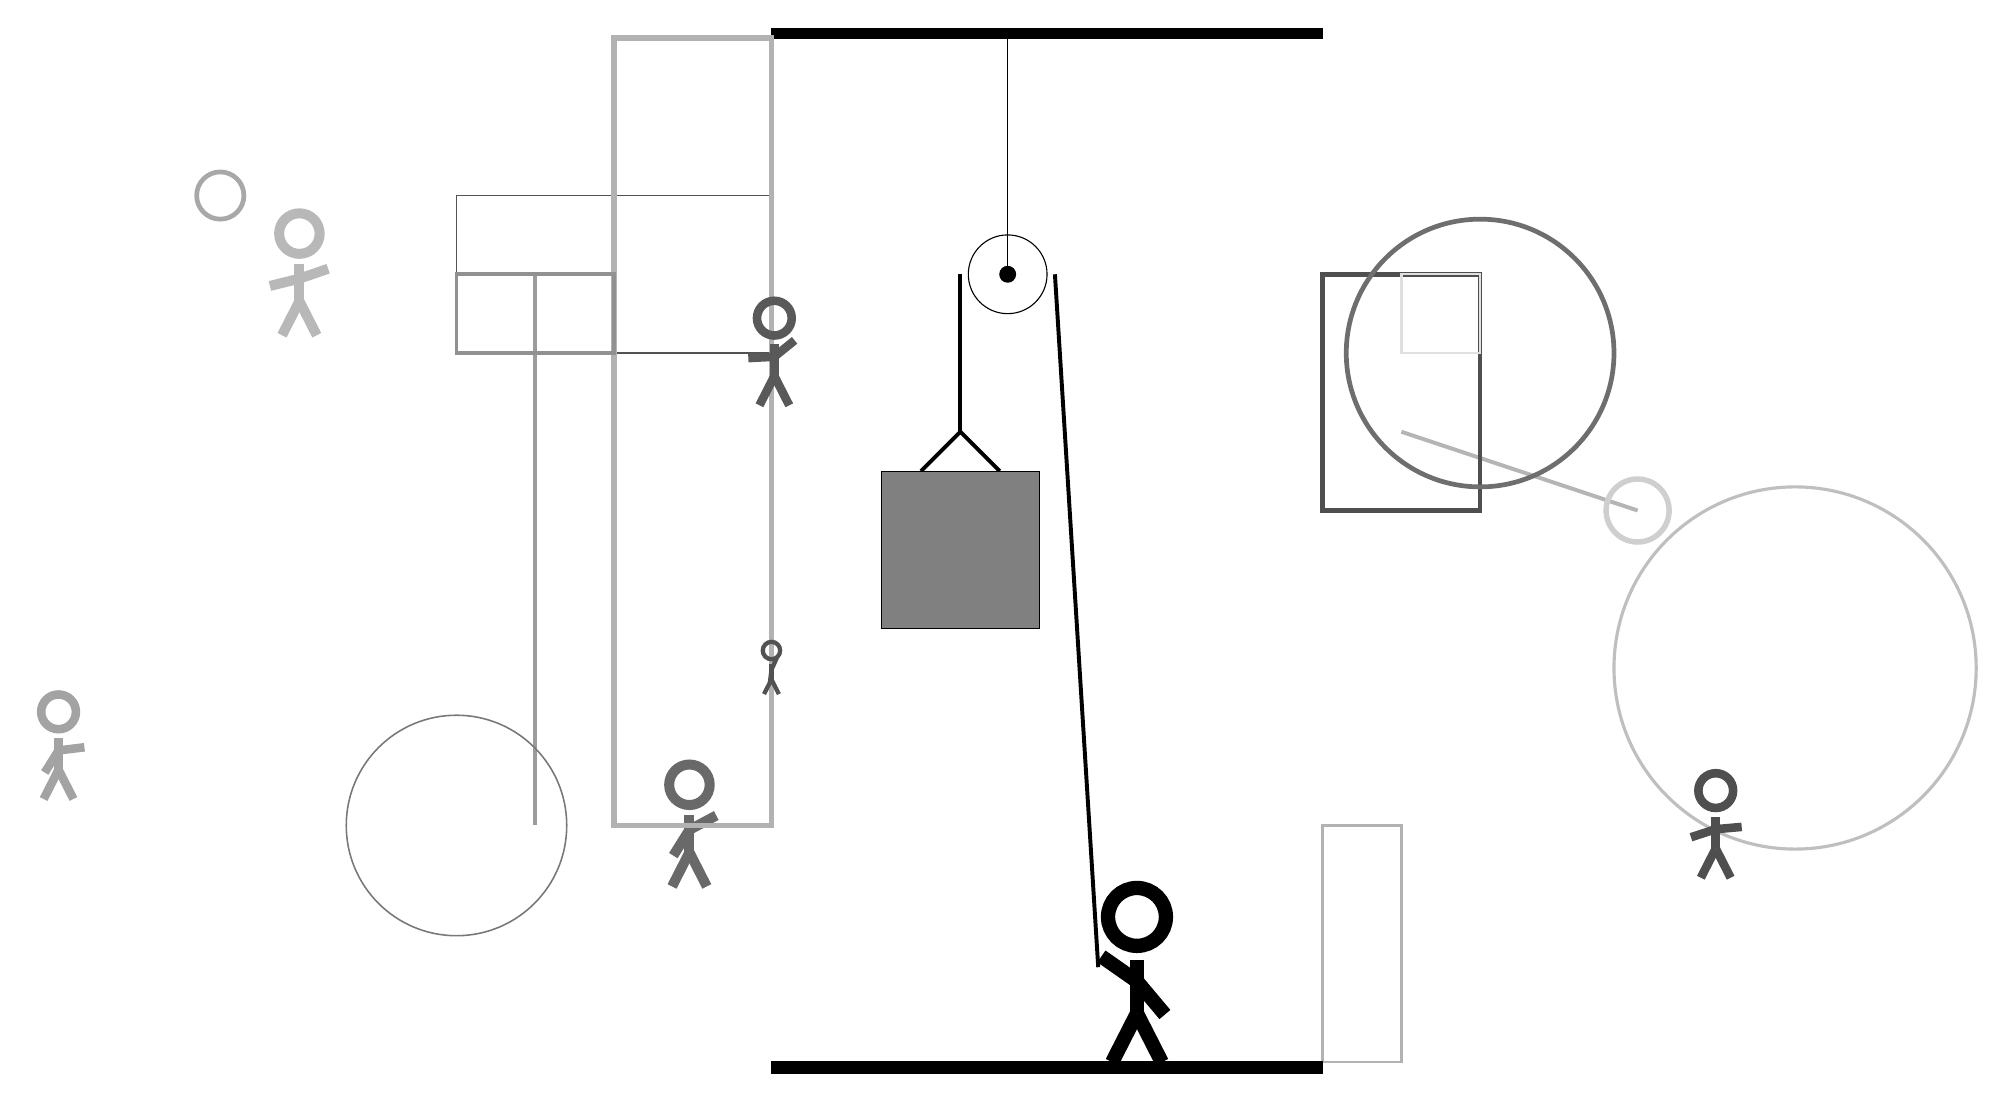
\begin{tikzpicture}
		%%%%% START %%%%%
		
		\draw[fill=black] (-2, 10) rectangle (5, 10.125);
		
		\draw (1, 7) circle (0.5);
		\draw[fill=black] (1, 7) circle (0.1);
		\draw (1, 10) -- (1, 7);
		
		\draw[line width=0.5mm] (-0.1, 4.5) -- (0.4, 5.0) -- (0.9, 4.5);
		\draw[fill=black!50] (-0.6, 4.5) rectangle (1.4, 2.5);
		
		\draw[line width=0.5mm] (0.4, 7) -- (0.4, 5.0);
		\centerarc[line width=0.5mm](1, 7)(0:180:0.6);
		\draw[line width=0.5mm](1.6, 7) -- (2.15, -1.8);
		
		\draw[line width=0.5mm, color=black!29](6, 5) -- (9, 4);
		
		\draw[line width=0.2mm, color=black!68] (-2, 6) rectangle (-6, 8);
		\node[line width=0.2mm, color=black!59] at (-3, 0) {\Strichmaxerl[7][58][28]};
		\draw [line width=0.4mm, color=black!25](11, 2) circle (2.3);
		\draw[line width=0.5mm, color=black!39](-5, 0) -- (-5, 7);
		\draw[line width=0.7mm, color=black!30] (-4, 10) rectangle (-2, 0);
		\draw [line width=0.7mm, color=black!19](9, 4) circle (0.4);
		
		\node[line width=0.6mm, color=black!68] at (-2, 2) {\Strichmaxerl[3][83][66]};
		\draw[line width=0.5mm, color=black!43] (-4, 7) rectangle (-6, 6);
		\node[line width=0.5mm, color=black!28] at (-8, 7) {\Strichmaxerl[7][14][19]};
		\draw[line width=0.6mm, color=black!69] (5, 7) rectangle (7, 4);
		\node[line width=0.7mm, color=black!36] at (-11, 1) {\Strichmaxerl[6][58][7]};
		\draw[line width=0.3mm, color=black!30] (5, 0) rectangle (6, -3);
		
		\draw [line width=0.6mm, color=black!34](-9, 8) circle (0.3);
		\node[line width=0.6mm, color=black!69] at (10, 0) {\Strichmaxerl[6][18][5]};
		\node[line width=0.4mm, color=black!65] at (-2, 6) {\Strichmaxerl[6][3][39]};
		
		\draw [line width=0.6mm, color=black!57](7, 6) circle (1.7);
		\draw[line width=0.3mm, color=black!12] (6, 7) rectangle (7, 6);
		\draw [line width=0.2mm, color=black!53](-6, 0) circle (1.4);
		
		
		\node at (2.6, -1.9) {\Strichmaxerl[10][-35][-50]};
		
		\draw[fill=black] (-2, -3) rectangle (5, -3.15);
		
		%%%%% END %%%%%
	\end{tikzpicture}
\end{document}